\chapter{Methodology}
\label{ch:intro}

\section{System Overview}

The architecture overview and the complete step-by-step algorithm flow of the proposed localization system are shown in Figure \ref{fig:diagram-map-basedlocalization} and Algorithm \ref{alg:localization-system}. The input of the system includes the raw online point-cloud, raw IMU data as well as the prior map , and output real-time accurate 6 DOF pose.\\	
The system can be divided in to the following different modules:
\begin{enumerate}
	\item Scan Pre-Processing: Performs a series of point cloud processing steps to filter and extract relevant features from the raw LiDAR data.
	
	\item LIDAR-INERTIA Odometry - Estimates high-frequency odometry by fusing raw IMU data and LiDAR scans. The resulting odometry is added as a local constraint (odom factor) to the factor graph.
	
	\item Dynamic Local Map Loader: Generates a local map around the robot’s current pose within a specified radius from the prior map.
	
	
	\item Scan-to-Map Matching: Aligns the current LiDAR scan with the local map to estimate the robot's pose in the prior map. The estimated pose is added as a prior constraint (map factor) to the factor graph.
	
	\item Sliding Window Factor Graph Optimizer:Fuses odometry and map constraints within a sliding window to optimize and output a real-time, accurate 6-DoF pose.
	
	
\end{enumerate}

\begin{figure}
    \centering
    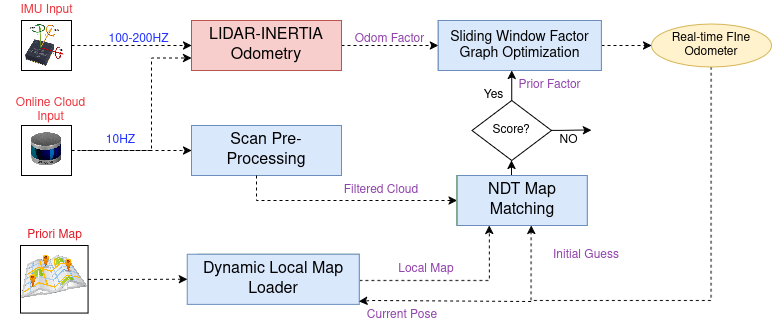
\includegraphics[width=1\linewidth]{images/system_overview.png}
    \caption{Complete Diagram of Map Based Localization}
    \label{fig:diagram-map-basedlocalization}
\end{figure}


\begin{algorithm}[H]
	\caption{LiDAR-Inertial Localization with Prior Map}
	\label{alg:localization-system}
	
	\textbf{Input:} $\mathcal{P}_t$ (LiDAR Point Cloud), $\mathcal{I}_t$ (IMU Data), $\mathcal{M}$ (Prior Map)\\
	\textbf{Output:} $\mathbf{T}_t$ (Real-time 6-DoF Pose)
	
	\begin{algorithmic}[1]
		
		\While{System is running}
		
		\State Acquire LiDAR point cloud $\mathcal{P}_t$ and IMU data $\mathcal{I}_t$
		
		\State Perform scan pre-processing on $\mathcal{P}_t$ to obtain filtered point cloud $\mathcal{P}_t^{filtered}$
		
		\State Estimate LiDAR-Inertial Odometry using $\{\mathcal{P}_t^{filtered}, \mathcal{I}_t\}$ to obtain odometry pose $\mathbf{T}_t^{lio}$	
		
		\If{$|| \mathbf{T}_t - \mathbf{T}_{last}^{map} || > d_{threshold}$}
		\State Load dynamic local map $\mathcal{M}_t^{local}$ from $\mathcal{M}$ centered at $\mathbf{T}_t^{lio}$
		\State Update $\mathbf{T}_{last}^{map} \gets \mathbf{T}_t$
		\EndIf
		
		\State Perform scan-to-map matching between $\mathcal{P}_t^{filtered}$ and $\mathcal{M}_t^{local}$ to obtain map-based pose $\mathbf{T}_t^{map}$
		
		\If{Matching score $> s_{threshold}$}
		\State Add prior factor with $\mathbf{T}_t^{map}$ to factor graph
		\EndIf
		
		\State Add odometry factor with $\mathbf{T}_t^{lio}$ to factor graph
		
		\State Optimize sliding window factor graph to obtain final pose $\mathbf{T}_t$
		
		\EndWhile
		
	\end{algorithmic}
\end{algorithm}


\section{LIDAR Scan Pre-Processing}
Before aligning each incoming LiDAR scan to the global map, we first subject the raw point cloud to a series of preprocessing operations. These operations improve both efficiency and reliability by filtering out irrelevant regions and outliers, downsampling to reduce data volume, and transforming the data into a consistent coordinate frame.Our approach, illustrated in Figure\ref{fig:lidar_scan_preprocessing}  consists of the following  main steps:
\begin{figure}
    \centering
    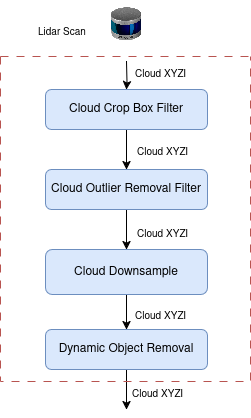
\includegraphics[width=0.4\linewidth]{images/LIDAR_PreProccess.drawio.png}
    \caption{LIDAR scan pre-processing}
    \label{fig:lidar_scan_preprocessing}
\end{figure}

\begin{itemize}
    \item \textbf{Crop-Box Filter}: This step confines the point cloud to a user-defined three-dimensional region (a bounding “box”) around the sensor or area of interest. By discarding all points lying outside this box, we focus only on the relevant portion of the scene, reducing both memory and computational overhead for subsequent processing.
    \item \textbf{Outlier Removal}: Once the point cloud is restricted to the area of interest, we remove random noise and spurious measurements using a statistical outlier filter. Concretely, we compute for each point the average distance to its k‐nearest neighbors. Points whose mean distance exceeds the global mean plus a chosen multiplier of the standard deviation are marked as outliers and deleted. This practice is a commonly adopted heuristic that discards stray or floating points, which might result from occasional sensor glitches or moving objects in the environment.
    \item \textbf{Voxel-Grid Downsampling} To further ease computational load, the point cloud is then downsampled. A typical approach uses a voxel-grid filter: space is subdivided into small volumetric “voxels,” and all points within each voxel are replaced by a single representative (often the centroid). This retains the main geometry while reducing point density, thereby speeding up map‐based matching algorithms.
    \item \textbf{Coordinate Transformation}:   Finally, we apply a rigid transformation that aligns the processed point cloud to a consistent coordinate frame used throughout our localization pipeline—the vehicle’s base link frame.This accounts for any known extrinsic offsets between the LiDAR sensor and the vehicle origin.
\end{itemize}

As summarized in Table~\ref{tab:lidar_preprocessing}, the LiDAR preprocessing parameters vary depending on the sensor type and application requirements. All filtering and scan processing operations are implemented using the Point Cloud Library (PCL).



\begin{table}[htbp]
\centering
\caption{LiDAR Scan Processing Methods and Parametrs  Across Different Sensor Setups}
\label{tab:lidar_preprocessing}
\begin{tabular}{|p{3.5cm}|p{3.5cm}|p{3.5cm}|p{3.5cm}|}
\hline
\textbf{Processing Step} & \textbf{KITTI(Velodyne HDL-64E)} & \textbf{MulRan(Ouster-OS1-64)} & \textbf{(Ouster-OS1-128)} \\
\hline
LiDAR Type & Velodyne HDL-64E & Ouster OS1-64 & Ouster OS1-128 \\
% \hline
% \textbf{Vertical Channels} & 64 & 64 & 128 \\
% \hline
% \textbf{Vertical FOV} & $\pm$2° to $\pm$24.8° ($\sim$26.8° total) & $\pm$16.6° ($\sim$33.2° total) & $\pm$22.5° ($\sim$45° total) \\
\hline
Max Range & $\sim$120 m & $\sim$120 m & $\sim$240 m \\
\hline
Crop Box Filter & 90-100m & 90-100m & 180-200m\\
\hline
Downsampling Method & Voxel-Grid(leaf-size: 0.5m) & Voxel-Grid(leaf-size: 0.4-0.6 m) & Voxel-Voxel(0.5-0.8 m) \\
\hline
Outlier Removal & Statistical (K=50, Std=1.0) & Statistical (K=40, Std=1.0) & Statistical(K=40 ,Std=1,0) \\
\hline
% \textbf{Ground Removal} & Not used & Yes — flat surface segmentation &  Yes — flat surface segmentation \\
% \hline
\end{tabular}
\end{table}

\section{Map Pre-Processing}

\subsubsection{Grid-based Point Map Cloud Division }

To efficiently handle high-resolution point cloud maps in large-scale localization, the global map is divided offline into smaller, manageable "tiles" based on a 2D grid as shown \ref{fig:pointcloud division}. Each point is assigned to a grid cell using its X and Y coordinates, grouping nearby points together. The grid size is user-defined, controlling the resolution of the division. Each grid cell is saved as an individual point cloud file, and its index is stored as metadata for fast retrieval. During localization, these indexes enable loading only the relevant grids within the robot's local map radius, reducing memory usage and improving processing efficiency.



\begin{figure}
    \centering
    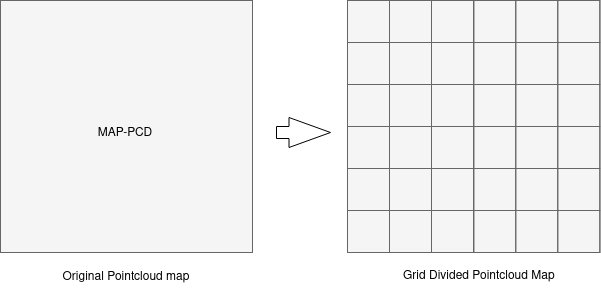
\includegraphics[width=0.8
    \linewidth]{images/map.drawio.png}
    \caption{Grid Based Point-cloud division }
    \label{fig:pointcloud division}
\end{figure}
\subsection{Dynamic Map Loading}

To enable scalable localization in large environments, a dynamic sub-map loading strategy is implemented based on the robot's motion and LiDAR characteristics. This approach ensures that only the necessary local grid tiles around the robot are loaded from the global prior map, reducing memory consumption and improving computational efficiency.

\begin{itemize}
	\item \textbf{Local Map Radius Determination:} 
	
	The radius of the local sub-map, denoted as $r_{map}$, defines the area around the robot within which map grids should be loaded. This radius is selected based on:
	
	\begin{itemize}
		\item LiDAR sensing range ($r_{lidar}$) — the effective field-of-view of the sensor.
		\item Safety margin ($r_{margin}$) — a user-defined buffer to ensure sufficient overlap for robust scan-to-map matching.
	\end{itemize}
	
	The total local map radius is computed as:
	
	\begin{equation}
		r_{map} = r_{lidar} + r_{margin}
	\end{equation}
	
	\item \textbf{Map Loading Condition:}
	
	The map is updated only when the robot moves beyond a predefined distance threshold $d_{thresh}$ from its last map update position $\mathbf{T}_{last}^{map}$. This prevents frequent reloading due to minor movements and ensures efficiency.
	
	The loading condition is defined as:
	
	\begin{equation}
		||\mathbf{T}_t - \mathbf{T}_{last}^{map}||_2 > d_{thresh}
	\end{equation}
	
	where:
	\begin{itemize}
		\item $\mathbf{T}_t$ is the current robot position.
		\item $|| \cdot ||_2$ denotes the Euclidean distance.
	\end{itemize}
	
	Once this condition is satisfied, the map loading process is triggered.
	
	\item \textbf{Selective Grid Loading and Unloading:}
	
	During map update, only the grids within the local map radius $r_{map}$ are loaded. Grids outside this radius, which are no longer within the robot's vicinity, are removed from memory to optimize resource usage.
	
	The procedure includes:
	\begin{itemize}
		\item Identify all grid cells within $r_{map}$ centered at $\mathbf{T}_t$.
		\item Load only the required grids from the global map $\mathcal{M}$ into the local map $\mathcal{M}_{t}^{local}$.
		\item Remove previously loaded grids that now lie outside $r_{map}$.
		\item Update the last map loading position: $\mathbf{T}_{last}^{map} \gets \mathbf{T}_t$.
	\end{itemize}
	
\end{itemize}


\subsection{LIDAR Inertia Odometry} 

\subsection{Scan-to-Map Matching}
\subsection{Scan-to-Map Matching Methodology}

The Scan-to-Map Matching module is a crucial component of the proposed localization system. Its primary objective is to align the current LiDAR scan with the dynamically loaded local map and estimate the robot's accurate pose within the prior map coordinate frame. 

In this work, the Normal Distributions Transform (NDT) algorithm is employed for robust and efficient scan registration. Specifically, a multi-threaded implementation of NDT (NDT-OMP) \cite{koide2019portable} is utilized, leveraging OpenMP-based parallelization to accelerate computation and enable real-time performance.

\begin{itemize}
	
	\item \textbf{NDT-based Scan Registration:}
	
	%The NDT algorithm represents the target map %$\mathcal{M}_t^{local}$ as a set of voxelized %grid cells, where each cell is modeled as a %Gaussian distribution with mean $\mu$ and %covariance $\Sigma$. The current LiDAR scan %$\mathcal{P}_t$ is aligned by estimating the %transformation parameters $\mathbf{T}_t = %[\mathbf{R}_t, \math
%	bf{t}_t]$ (rotation and translation) that %maximize the likelihood of scan points given the %map distributions.
	
	The scan registration problem is formulated as minimizing the negative log-likelihood:
	
	\begin{equation}
		\mathbf{T}_t^* = \arg\min_{\mathbf{T}_t} \sum_{x \in \mathcal{P}_t} - \log p( \mathbf{T}_t x )
	\end{equation}
	
	where $p( \mathbf{T}_t x )$ is the probability density of a transformed scan point $x$ within the corresponding Gaussian of the map voxel.
	
	The optimization is performed using Newton’s method, utilizing the gradient and Hessian derived from the objective function.
	
	\item \textbf{Implementation Details:}
	
	In this thesis, the NDT-OMP library \cite{koide2019portable} is integrated due to its superior multi-threaded performance. Additionally, Autoware's NDT scan matcher \cite{autoware_ndt} is used for parameter tuning and system validation.
	
	The NDT parameters are configured as follows:
	\begin{itemize}
		\item Voxel Grid Resolution: User-defined (e.g., 1.0 m)
		\item Maximum Iterations: 30 -- 50
		\item Convergence Threshold: 1e-6
		\item Number of Threads: Dynamic (depending on CPU cores)
	\end{itemize}
	
	\item \textbf{Pose Fusion:}
	
	The resulting pose estimate from NDT matching, denoted as $\mathbf{T}_t^{map}$, is integrated into the sliding window factor graph as a prior constraint (map factor), complementing the high-frequency odometry from the LiDAR-Inertial Odometry (LIO) module.
	
\end{itemize}



\section{Fusion}

The fusion strategy combines high-frequency odometry from LIO with global pose corrections from scan-to-map matching. An incremental solver (iSAM2) with fixed-lag smoothing is used to maintain real-time performance while optimizing recent trajectory estimates. This approach ensures accurate and drift-resilient pose estimation while keeping computational cost bounded.

\subsection{Factor Graph Formulation}

We denote the robot trajectory as a sequence of poses:
\begin{equation}
	\mathcal{X} = { \mathbf{x}_0, \mathbf{x}_1, \dots, \mathbf{x}_k }, \quad \mathbf{x}_i \in SE(3)
\end{equation}
where each pose $\mathbf{x}i $  represents the 6-DOF position and orientation of the robot at discrete time step \textit{i} , and SE(3) denotes the special Euclidean group representing 3D rigid body transformations.

\paragraph{1. Prior Factor}
A prior factor is used to anchor the initial pose to a known global reference frame. It models the prior distribution over the initial state , expressed as:
\begin{equation}
	\phi_{\text{prior}}(\mathbf{x}_0) = \exp\left( -\frac{1}{2} | \mathbf{x}_0 - \bar{\mathbf{x}}_0 |^2{\Sigma_0} \right)
\end{equation}

In this formulation, $\mathbf{x}_0$ is the estimated initial pose of the robot. The term $\bar{\mathbf{x}}_0$ denotes the prior mean pose from the first LIO output or initialization, and $\mathbf{{\Sigma_0}}$ is the prior covariance matrix reflecting the uncertainty in. This Gaussian prior serves as a fixed anchor to stabilize the trajectory estimation.

\paragraph{2. Odometry (Between) Factors}
Relative motion from LIO is encoded using between factors, which represent the relative transformation between consecutive poses:
\begin{equation}
	\phi_{\text{odom}}(\mathbf{x}{i-1}, \mathbf{x}i) = \exp\left( -\frac{1}{2} \left| f{\text{odom}}(\mathbf{x}_{i-1}, \mathbf{x}i) - \bar{\mathbf{z}}i^{\text{odom}} \right|^2{\Sigma{\text{odom}}} \right)
\end{equation}
Here,$\bar{\mathbf{z}}i^{\text{odom}}$ is the relative pose measurement between time steps $\text{\textit{i}}$  and $\text{\textit{i+1}}$, derived from the LIO module. The $f{\text{odom}(\mathbf{.})}$
function  calculates the predicted relative transformation between the estimated poses $\mathbf{x}_{i-1}$ and $\mathbf{x}_{i},$ . The $ \mathbf{\Sigma{\text{odom}}}$ term   is the associated covariance matrix, which quantifies the uncertainty in the odometry measurement. These between factors form the sequential backbone of the trajectory by chaining consecutive pose estimates together through relative motion constraints.

\paragraph{3. Map-Matching Priors}
Absolute pose estimates derived from scan-to-map matching using Normal Distributions Transform (NDT) are incorporated as prior constraints on select poses:
\begin{equation}
	\phi_{\text{map}}(\mathbf{x}_j) = \exp\left( -\frac{1}{2} | \mathbf{x}j - \bar{\mathbf{x}}j^{\text{map}} |^2{\Sigma{\text{map}}} \right)
\end{equation}
In this expression, $\bar{\mathbf{x}}j^{\text{map}} $  denotes the global pose obtained by aligning the current LiDAR scan with a pre-built prior map using scan matching techniques. The associated covariance matrix $\mathbf{\Sigma{\text{map}}}$ expresses the uncertainty of the registration process, accounting for alignment quality and sensor noise. These priors provide absolute spatial constraints within the factor graph, which help to correct accumulated drift from relative odometry and enhance the global consistency of the trajectory estimation.
\subsection{Maximum A Posteriori (MAP) Estimation}

The objective of the sensor fusion system is to compute the most probable robot trajectory given all available measurements, including odometry and map-matching observations. This is formulated as a Maximum A Posteriori (MAP) estimation problem, expressed as the following nonlinear least-squares objective:

\begin{equation}
	\mathbf{X}^* = \arg\min_{\mathbf{X}} \left(
	\| \mathbf{x}_0 - \bar{\mathbf{x}}_0 \|^2_{\Sigma_0} +
	\sum_{i=1}^{k} \left\| f_{\text{odom}}(\mathbf{x}_{i-1}, \mathbf{x}_i) - \bar{\mathbf{z}}_i^{\text{odom}} \right\|^2_{\Sigma_{\text{odom}}} +
	\sum_{j \in \mathcal{M}} \left\| \mathbf{x}_j - \bar{\mathbf{x}}_j^{\text{map}} \right\|^2_{\Sigma_{\text{map}}}
	\right)
	\label{eq:map-estimation}
\end{equation}

\begin{comment}
	Here:
	\begin{itemize}
		\item \( \mathbf{X} = \{ \mathbf{x}_0, \mathbf{x}_1, \dots, \mathbf{x}_k \} \) is the sequence of robot poses to be estimated.
		\item \( \bar{\mathbf{x}}_0 \) is the prior estimate of the initial pose, with covariance \( \Sigma_0 \).
		\item \( \bar{\mathbf{z}}_i^{\text{odom}} \) is the observed relative transformation between \( \mathbf{x}_{i-1} \) and \( \mathbf{x}_i \) from LiDAR-inertial odometry, with associated covariance \( \Sigma_{\text{odom}} \).
		\item \( f_{\text{odom}}(\cdot) \) is the motion model predicting the relative transformation between consecutive poses.
		\item \( \bar{\mathbf{x}}_j^{\text{map}} \) represents the pose obtained from map-matching at selected indices \( j \in \mathcal{M} \), with uncertainty \( \Sigma_{\text{map}} \).
	\end{itemize}
\end{comment}

Each term in the cost function represents a Mahalanobis distance, penalizing deviations from the respective measurements weighted by their uncertainty. Solving this objective yields the optimal trajectory estimate \( \mathbf{X}^* \), which fuses relative odometry and global pose observations in a probabilistically consistent manner.


\subsection{Fixed-Lag Smoothing and Marginalization}

In our proposed system, fixed-lag smoothing is used to maintain real-time performance while optimizing the recent trajectory of the robot. Instead of keeping the entire history of poses in the factor graph, we define a sliding time window of length \( \tau \), such that only poses within the interval \( [t_k - \tau, t_k] \) are retained, where \( t_k \) is the current time. This ensures that the graph grows only within a fixed temporal horizon, regardless of how long the system has been running.

Let \( \mathbf{x}_0, \mathbf{x}_1, \dots, \mathbf{x}_k \) represent the sequence of robot poses over time. At each time step, the latest pose \( \mathbf{x}_k \) is added to the factor graph along with new factors derived from LIO (odometry) and map-matching. Older poses such as \( \mathbf{x}_i \) for which \( t_i < t_k - \tau \) are marginalized out to limit the graph size.

The process of marginalization involves removing a variable (pose) from the graph while preserving its influence on the remaining variables. Suppose the state vector is partitioned as:
\begin{equation}
	\mathbf{x} = \begin{bmatrix} \mathbf{x}_m \\ \mathbf{x}_r \end{bmatrix},
\end{equation}
where \( \mathbf{x}_m \) are the variables to be marginalized (e.g., old poses outside the lag window), and \( \mathbf{x}_r \) are the variables retained in the active window. The joint probability distribution is expressed as:
\begin{equation}
	P(\mathbf{x}_m, \mathbf{x}_r) = P(\mathbf{x}_m | \mathbf{x}_r) P(\mathbf{x}_r).
\end{equation}
To obtain a reduced representation, we marginalize out \( \mathbf{x}_m \):
\begin{equation}
	P(\mathbf{x}_r) = \int P(\mathbf{x}_m, \mathbf{x}_r) \, d\mathbf{x}_m.
\end{equation}

GTSAM uses the Schur complement to perform this marginalization operation. As a result, a new dense factor is introduced between variables in \( \mathbf{x}_r \) that were connected to \( \mathbf{x}_m \), preserving the influence of the eliminated variables.

\begin{figure}[htbp]
	\centering
	\begin{subfigure}[b]{0.5\textwidth}
		\centering
		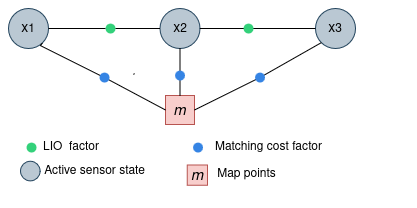
\includegraphics[width=\textwidth]{images/fixed_lag_smooth_a.png}
		 \captionsetup{width=2\textwidth}
		\caption{The initial factor graph contains active states \( \mathbf{x}_1 \) to \( \mathbf{x}_3 \), linked through LiDAR-inertial odometry (LIO) and map-matching factors. }
		\label{fig:bayes-a}
	\end{subfigure}
		\vskip\baselineskip
	\begin{subfigure}[b]{0.5\textwidth}
		\centering
		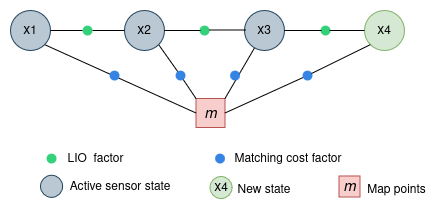
\includegraphics[width=\textwidth]{images/fixed_lag_smooth_b.png}
		\captionsetup{width=2\textwidth}
		\caption{A new state \( \mathbf{x}_4 \) is introduced, remaining within the lag window. }
		\label{fig:bayes-b}
	\end{subfigure}
	\vskip\baselineskip
	\begin{subfigure}[b]{0.7\textwidth}
		\centering
		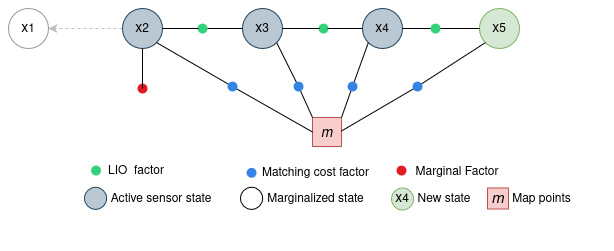
\includegraphics[width=\textwidth]{images/fixed_lag_smooth_c.png}
		\captionsetup{width=1.2\textwidth}
		
		\caption{As state \( \mathbf{x}_5 \) is added, the oldest state \( \mathbf{x}_1 \) is marginalized and its influence is preserved via a prior factor. 
		}
		\label{fig:bayes-c}
	\end{subfigure}
    \vskip\baselineskip
	\begin{subfigure}[b]{0.7\textwidth}
		\centering
		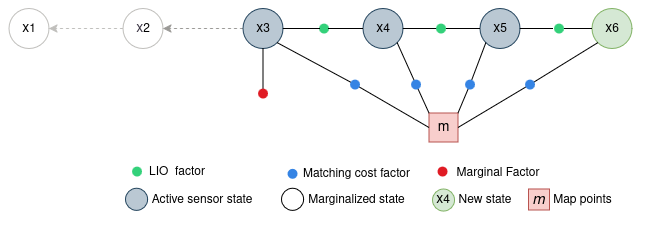
\includegraphics[width=\textwidth]{images/fixed_lag_smooth_d.png}
		\captionsetup{width=1.2\textwidth}
		\caption{At time \( t_6 \), \( \mathbf{x}_6 \) is introduced and \( \mathbf{x}_2 \) is marginalized, maintaining a fixed-lag window over the most recent four states. 
	}
		\label{fig:bayes-d}
	\end{subfigure}
    \vskip\baselineskip
	\caption{Demonstration of fixed-lag smoothing with a lag size of \( n = 4 \) in a factor graph-based localization system.}
	\label{fig:fixed-lag-example}
\end{figure}

The process of fixed-lag smoothing is illustrated in Figure~\ref{fig:fixed-lag-example} using a temporal window of length \( n = 4 \). Initially (Figure~\ref{fig:bayes-a}), the system contains states \( \mathbf{x}_1 \), \( \mathbf{x}_2 \), and \( \mathbf{x}_3 \), connected by odometry and map-matching factors. As pose \( \mathbf{x}_4 \) is added at time \( t_4 \) (Figure~\ref{fig:bayes-b}), it links to \( \mathbf{x}_3 \) through a new odometry factor and includes a map constraint. Since all poses \( \mathbf{x}_1 \) to \( \mathbf{x}_4 \) lie within the lag window \( [t_1, t_4] \), the graph remains fully active and no marginalization occurs.


When the system reaches time step \( t_5 \), pose \( \mathbf{x}_5 \) is added, along with its corresponding odometry and map-matching constraints. At this point, pose \( \mathbf{x}_1 \) falls outside the fixed-lag window \( [t_2, t_5] \). As a result, it is marginalized. This process eliminates \( \mathbf{x}_1 \) from the graph but replaces its influence with a dense prior that connects to the remaining relevant states, particularly \( \mathbf{x}_2 \) and beyond (Figure~\ref{fig:bayes-c}). The marginalized node is no longer directly optimized, but its effect is preserved through conditional probability in the form of a Bayes net.

At the next step, time \( t_6 \), a new pose \( \mathbf{x}_6 \) is introduced. To maintain the lag window \( [t_3, t_6] \), the system marginalizes pose \( \mathbf{x}_2 \), introducing another dense factor that connects to the active variables. The current active states now consist of \( \mathbf{x}_3 \), \( \mathbf{x}_4 \), \( \mathbf{x}_5 \), and \( \mathbf{x}_6 \), all within the sliding lag window (Figure~\ref{fig:bayes-d}).

This incremental update mechanism, implemented using the GTSAM library, maintains a bounded graph size by marginalizing old variables into Bayes net conditionals while preserving historical information. Recent poses within the active window are kept in a factor graph and updated via iSAM2, striking a balance between computational efficiency and estimation accuracy for real-time localization.


\section{Dynamic Object Detection and Removal}

\subsection{Dynamic Object Detection}

To identify and remove dynamic objects from the LiDAR point cloud, this work utilizes a deep learning-based 3D object detection pipeline based on CenterPoint\cite{yin2021center}. The model is developed and trained using the MMDetection3D framework\cite{mmdet3d2020}, and is deployed for real-time inference using the Autoware-compatible implementation\cite{autoware_universe}.

The detection architecture adopts the two-stage design of CenterPoint\cite{yin2021center}, as shown in Figure \ref{fig:Overview-CenterPoint }. First, the raw LiDAR point cloud is voxelized and processed by a voxel feature encoder and a PointPillars-based sparse convolutional backbone\cite{lang2019pointpillars}, which extracts high-level spatial features. These features are projected into a Bird’s-Eye View (BEV) map, enabling efficient object detection. A keypoint-based detection head then identifies object centers and regresses 3D bounding box attributes, including size, orientation, and velocity. The final output includes class-labeled 3D detections, which are used to support dynamic object removal.

Instead of training from scratch, this work utilizes a pretrained CenterPoint model trained on the nuScenes dataset \cite{caesar2020nuscenes}, comprising over 28k LiDAR frames. The model includes five object classes: CAR, TRUCK, BUS, BICYCLE, and PEDESTRIAN. These categories cover the primary dynamic agents present in urban driving scenarios. After training, the model is exported to the ONNX (Open Neural Network Exchange) format, which supports cross-platform deployment and enables hardware-accelerated inference using TensorRT.




\subsection{Detected Object removal }

Following object detection, dynamic elements are removed from the LiDAR point cloud using their predicted 3D bounding boxes. For each detected object, its position, dimensions, and orientation are used to define an oriented 3D cropping volume. These bounding boxes are expanded slightly with a fixed margin to ensure full exclusion of the object’s points, accounting for detection uncertainty or sensor noise.

Each bounding box is then used to define a geometric filter in 3D space. The removal process involves identifying all LiDAR points that fall within the transformed bounding box and excluding them from the original scan. This is performed iteratively for all detected dynamic objects in each frame. The result is a filtered point cloud that retains only static environmental features, which are then used for downstream localization tasks. 









